%%%%%%%%%%%%%%%%%%%%%%%%%%%%%%%%%%%%%%%%%
%  My documentation report
%  Objetive: Explain what I did and how, so someone can continue with the investigation
%
% Important note:
% Chapter heading images should have a 2:1 width:height ratio,
% e.g. 920px width and 460px height.
%
%%%%%%%%%%%%%%%%%%%%%%%%%%%%%%%%%%%%%%%%%

%----------------------------------------------------------------------------------------
%	PACKAGES AND OTHER DOCUMENT CONFIGURATIONS
%----------------------------------------------------------------------------------------

\documentclass[11pt,fleqn,twocolumn]{book} % Default font size and left-justified equations

\usepackage[top=3cm,bottom=3cm,left=2.5cm,right=2.5cm,headsep=10pt,letterpaper]{geometry} % Page margins
\usepackage{booktabs}

\usepackage{longtable}

\usepackage{afterpage}
\usepackage[table,xcdraw]{xcolor}
\usepackage{xcolor,lipsum} % Required for specifying colors by name
\definecolor{ocre}{RGB}{51,102,0} 
\definecolor{lightgray}{RGB}{229,229,229} 
% Font Settings
\usepackage{avant} % Use the Avantgarde font for headings
%\usepackage{times} % Use the Times font for headings
\usepackage{mathptmx} % Use the Adobe Times Roman as the default text font together with math symbols from the Sym­bol, Chancery and Com­puter Modern fonts

\setlength\columnsep{43pt} % This is the default columnsep for all pages
%\columnsep{10pt} 
\usepackage{microtype} % Slightly tweak font spacing for aesthetics
\usepackage[utf8]{inputenc} % Required for including letters with accents
\usepackage[T1]{fontenc} % Use 8-bit encoding that has 256 glyphs

\usepackage{verbatim}

% autor a la derecha en poema
\usepackage{ragged2e}
% MATHS PACKAGE
\usepackage{amsmath,tikz}
\usetikzlibrary{matrix}
\newcommand*{\horzbar}{\rule[0.05ex]{2.5ex}{0.5pt}}
\usepackage{calc}

% VERBATIM PACKAGE
\usepackage{verbatim}

% Bibliography
\usepackage[style=alphabetic,sorting=nyt,sortcites=true,autopunct=true,babel=hyphen,hyperref=true,abbreviate=false,backref=true,backend=biber]{biblatex}
\addbibresource{bibliography.bib} % BibTeX bibliography file
\defbibheading{bibempty}{}

%----------------------------------------------------------------------------------------
%	VARIOUS REQUIRED PACKAGES
%----------------------------------------------------------------------------------------

\usepackage{titlesec} % Allows customization of titles

\usepackage{graphicx} % Required for including pictures
\graphicspath{{Pictures/}} % Specifies the directory where pictures are stored

\usepackage{lipsum} % Inserts dummy text

\usepackage{tikz} % Required for drawing custom shapes

\usepackage[english]{babel} % English language/hyphenation
%\usepackage[spanish]{babel}
\usepackage{enumitem} % Customize lists
\setlist{nolistsep} % Reduce spacing between bullet points and numbered lists

\usepackage{booktabs} % Required for nicer horizontal rules in tables

\usepackage{eso-pic} % Required for specifying an image background in the title page

%----------------------------------------------------------------------------------------
%	MAIN TABLE OF CONTENTS
%----------------------------------------------------------------------------------------

\usepackage{titletoc} % Required for manipulating the table of contents

\contentsmargin{0cm} % Removes the default margin
% Chapter text styling
\titlecontents{chapter}[1.25cm] % Indentation
{\addvspace{15pt}\large\sffamily\bfseries} % Spacing and font options for chapters
{\color{ocre!60}\contentslabel[\Large\thecontentslabel]{1.25cm}\color{ocre}} % Chapter number
{}  
{\color{ocre!60}\normalsize\sffamily\bfseries\;\titlerule*[.5pc]{.}\;\thecontentspage} % Page number
% Section text styling
\titlecontents{section}[1.25cm] % Indentation
{\addvspace{5pt}\sffamily\bfseries} % Spacing and font options for sections
{\contentslabel[\thecontentslabel]{1.25cm}} % Section number
{}
{\sffamily\hfill\color{black}\thecontentspage} % Page number
[]
% Subsection text styling
\titlecontents{subsection}[1.25cm] % Indentation
{\addvspace{1pt}\sffamily\small} % Spacing and font options for subsections
{\contentslabel[\thecontentslabel]{1.25cm}} % Subsection number
{}
{\sffamily\;\titlerule*[.5pc]{.}\;\thecontentspage} % Page number
[] 

%----------------------------------------------------------------------------------------
%	MINI TABLE OF CONTENTS IN CHAPTER HEADS
%----------------------------------------------------------------------------------------

% Section text styling
\titlecontents{lsection}[0em] % Indendating
{\footnotesize\sffamily} % Font settings
{}
{}
{}

% Subsection text styling
\titlecontents{lsubsection}[.5em] % Indentation
{\normalfont\footnotesize\sffamily} % Font settings
{}
{}
{}
 
%----------------------------------------------------------------------------------------
%	PAGE HEADERS
%----------------------------------------------------------------------------------------

\usepackage{fancyhdr} % Required for header and footer configuration

\pagestyle{fancy}

\addto\captionsenglish{\renewcommand{\chaptername}{Lección}}
\renewcommand{\chaptermark}[1]{\markboth{\sffamily\normalsize\bfseries\chaptername\ \thechapter.\ #1}{}} % Chapter text font settings
\renewcommand{\sectionmark}[1]{\markright{\sffamily\normalsize\thesection\hspace{5pt}#1}{}} % Section text font settings
\fancyhf{} \fancyhead[LE,RO]{\sffamily\normalsize\thepage} % Font setting for the page number in the header
\fancyhead[LO]{\rightmark} % Print the nearest section name on the left side of odd pages
\fancyhead[RE]{\leftmark} % Print the current chapter name on the right side of even pages
\renewcommand{\headrulewidth}{0.5pt} % Width of the rule under the header
\addtolength{\headheight}{2.5pt} % Increase the spacing around the header slightly
\renewcommand{\footrulewidth}{0pt} % Removes the rule in the footer
\fancypagestyle{plain}{\fancyhead{}\renewcommand{\headrulewidth}{0pt}} % Style for when a plain pagestyle is specified

% Removes the header from odd empty pages at the end of chapters
\makeatletter
\renewcommand{\cleardoublepage}{
\clearpage\ifodd\c@page\else
\hbox{}
\vspace*{\fill}
\thispagestyle{empty}
\newpage
\fi}

%----------------------------------------------------------------------------------------
%	THEOREM STYLES
%----------------------------------------------------------------------------------------

\usepackage{amsmath,amsfonts,amssymb,amsthm} % For math equations, theorems, symbols, etc

\newcommand{\intoo}[2]{\mathopen{]}#1\,;#2\mathclose{[}}
\newcommand{\ud}{\mathop{\mathrm{{}d}}\mathopen{}}
\newcommand{\intff}[2]{\mathopen{[}#1\,;#2\mathclose{]}}
\newtheorem{notation}{Notation}[chapter]

%%%%%%%%%%%%%%%%%%%%%%%%%%%%%%%%%%%%%%%%%%%%%%%%%%%%%%%%%%%%%%%%%%%%%%%%%%%
%%%%%%%%%%%%%%%%%%%% dedicated to boxed/framed environements %%%%%%%%%%%%%%
%%%%%%%%%%%%%%%%%%%%%%%%%%%%%%%%%%%%%%%%%%%%%%%%%%%%%%%%%%%%%%%%%%%%%%%%%%%
\newtheoremstyle{ocrenumbox}% % Theorem style name
{5pt}% Space above
{5pt}% Space below
{\small\sffamily}% % Body font
{}% Indent amount
{\small\bf\sffamily\color{ocre}}% % Theorem head font
{\;}% Punctuation after theorem head
{0.25em}% Space after theorem head
{\normalsize\sffamily\color{ocre}\thmname{#1}\nobreakspace\thmnumber{\@ifnotempty{#1}{}\@upn{#2}}% Theorem text (e.g. Theorem 2.1)
\thmnote{\nobreakspace\the\thm@notefont\sffamily\bfseries\color{black}---\nobreakspace#3.}} % Optional theorem note
\renewcommand{\qedsymbol}{$\blacksquare$}% Optional qed square

\newtheoremstyle{blacknumex}% Theorem style name
{5pt}% Space above
{5pt}% Space below
{\normalfont}% Body font
{} % Indent amount
{\small\bf\sffamily}% Theorem head font
{\;}% Punctuation after theorem head
{0.25em}% Space after theorem head
{\small\sffamily{\tiny\ensuremath{\blacksquare}}\nobreakspace\thmname{#1}\nobreakspace\thmnumber{\@ifnotempty{#1}{}\@upn{#2}}% Theorem text (e.g. Theorem 2.1)
\thmnote{\nobreakspace\the\thm@notefont\sffamily\bfseries---\nobreakspace#3.}}% Optional theorem note

\newtheoremstyle{blacknumbox} % Estilo de Sabías qué? y Para tener en cuenta 
{0pt}% Space above
{0pt}% Space below
{\small\sffamily}% Body font
{}% Indent amount
{\small\bf\sffamily}% Theorem head font
{\;}% Punctuation after theorem head
{0.25em}% Space after theorem head
{\normalsize\sffamily\thmname{#1}\nobreakspace\thmnumber{\@ifnotempty{#1}{}\@upn{#2}}% Theorem text (e.g. Theorem 2.1)
\thmnote{\nobreakspace\the\thm@notefont\sffamily\bfseries---\nobreakspace#3.}}% Optional theorem note

%%%%%%%%%%%%%%%%%%%%%%%%%%%%%%%%%%%%%%%%%%%%%%%%%%%%%%%%%%%%%%%%%%%%%%%%%%%
%%%%%%%%%%%%% dedicated to non-boxed/non-framed environements %%%%%%%%%%%%%
%%%%%%%%%%%%%%%%%%%%%%%%%%%%%%%%%%%%%%%%%%%%%%%%%%%%%%%%%%%%%%%%%%%%%%%%%%%
\newtheoremstyle{ocrenum}% % Theorem style name
{5pt}% Space above
{5pt}% Space below
{\normalfont}% % Body font
{}% Indent amount
{\small\bf\sffamily\color{ocre}}% % Theorem head font
{\;}% Punctuation after theorem head
{0.25em}% Space after theorem head
{\small\sffamily\color{ocre}\thmname{#1}\nobreakspace\thmnumber{\@ifnotempty{#1}{}\@upn{#2}}% Theorem text (e.g. Theorem 2.1)
\thmnote{\nobreakspace\the\thm@notefont\sffamily\bfseries\color{black}---\nobreakspace#3.}} % Optional theorem note
\renewcommand{\qedsymbol}{$\blacksquare$}% Optional qed square
\makeatother

% Defines the theorem text style for each type of theorem to one of the three styles above
%\newcounter{dummy} 
%\numberwithin{dummy}{section}
\theoremstyle{ocrenumbox}
\newtheorem*{theoremeT}{En esta lección:\\}
\newtheorem*{problem}{Problem}
\newtheorem*{exerciseT}{Taller\\}
\theoremstyle{blacknumex}
\newtheorem*{exampleT}{Example}
\theoremstyle{blacknumbox}
\newtheorem*{vocabulary}{Vocabulary}
\newtheorem*{definitionT}{Sabías qué?}
\newtheorem*{corollaryT}{Para tener en cuenta\\}
\theoremstyle{ocrenum}
\newtheorem*{proposition}{Proposition}

%----------------------------------------------------------------------------------------
%	DEFINITION OF COLORED BOXES
%----------------------------------------------------------------------------------------

\RequirePackage[framemethod=default]{mdframed} % Required for creating the theorem, definition, exercise and corollary boxes

% Theorem box
\newmdenv[skipabove=7pt,
skipbelow=7pt,
backgroundcolor=black!5,
linecolor=ocre,
innerleftmargin=5pt,
innerrightmargin=5pt,
innertopmargin=5pt,
leftmargin=0cm,
rightmargin=0cm,
innerbottommargin=5pt]{tBox}

% Exercise box	  
\newmdenv[skipabove=7pt,
skipbelow=7pt,
rightline=false,
leftline=true,
topline=false,
bottomline=false,
backgroundcolor=ocre!10,
linecolor=ocre,
innerleftmargin=5pt,
innerrightmargin=5pt,
innertopmargin=5pt,
innerbottommargin=5pt,
leftmargin=0cm,
rightmargin=0cm,
linewidth=4pt]{eBox}	

% Definition box
\newmdenv[skipabove=7pt,
skipbelow=7pt,
rightline=false,
leftline=true,
topline=false,
bottomline=false,
linecolor=ocre,
innerleftmargin=5pt,
innerrightmargin=5pt,
innertopmargin=0pt,
leftmargin=0cm,
rightmargin=0cm,
linewidth=4pt,
innerbottommargin=0pt]{dBox}	

% Corollary box
\newmdenv[skipabove=7pt,
skipbelow=7pt,
rightline=true,
leftline=true,
topline=true,
bottomline=true,
linecolor=teal,
backgroundcolor=teal!20,
innerleftmargin=5pt,
innerrightmargin=5pt,
innertopmargin=5pt,
leftmargin=0cm,
rightmargin=0cm,
linewidth=4pt,
innerbottommargin=5pt]{cBox}

% Creates an environment for each type of theorem and assigns it a theorem text style from the "Theorem Styles" section above and a colored box from above
\newenvironment{theorem}{\begin{tBox}\begin{theoremeT}}{\end{theoremeT}\end{tBox}}
\newenvironment{exercise}{\begin{eBox}\begin{exerciseT}}{\hfill{\color{ocre}\tiny\ensuremath{\blacksquare}}\end{exerciseT}\end{eBox}}				  
\newenvironment{definition}{\begin{dBox}\begin{definitionT}}{\end{definitionT}\end{dBox}}
%\newenvironment{sabias}{\begin{dBox}\begin{sabias}}{\end{sabias}\end{dBox}}	
\newenvironment{example}{\begin{exampleT}}{\hfill{\tiny\ensuremath{\blacksquare}}\end{exampleT}}		
\newenvironment{corollary}{\begin{cBox}\begin{corollaryT}}{\end{corollaryT}\end{cBox}}	

%----------------------------------------------------------------------------------------
%	REMARK ENVIRONMENT
%----------------------------------------------------------------------------------------

\newenvironment{remark}{\par\vspace{10pt}\small % Vertical white space above the remark and smaller font size
\begin{list}{}{
\leftmargin=35pt % Indentation on the left
\rightmargin=25pt}\item\ignorespaces % Indentation on the right
\makebox[-2.5pt]{\begin{tikzpicture}[overlay]
\node[draw=ocre!60,line width=1pt,circle,fill=ocre!25,font=\sffamily\bfseries,inner sep=2pt,outer sep=0pt] at (-15pt,0pt){\textcolor{ocre}{R}};\end{tikzpicture}} % Orange R in a circle
\advance\baselineskip -1pt}{\end{list}\vskip5pt} % Tighter line spacing and white space after remark

%----------------------------------------------------------------------------------------
%	SECTION NUMBERING IN THE MARGIN
%----------------------------------------------------------------------------------------

\makeatletter
\renewcommand{\@seccntformat}[1]{\llap{\textcolor{ocre}{\csname the#1\endcsname}\hspace{1em}}}                    
\renewcommand{\section}{\@startsection{section}{1}{\z@}
{-4ex \@plus -1ex \@minus -.4ex}
{1ex \@plus.2ex }
{\normalfont\large\sffamily\bfseries}}
\renewcommand{\subsection}{\@startsection {subsection}{2}{\z@}
{-3ex \@plus -0.1ex \@minus -.4ex}
{0.5ex \@plus.2ex }
{\normalfont\sffamily\bfseries}}
\renewcommand{\subsubsection}{\@startsection {subsubsection}{3}{\z@}
{-2ex \@plus -0.1ex \@minus -.2ex}
{.2ex \@plus.2ex }
{\normalfont\small\sffamily\bfseries}}                        
\renewcommand\paragraph{\@startsection{paragraph}{4}{\z@}
{-2ex \@plus-.2ex \@minus .2ex}
{.1ex}
{\normalfont\small\sffamily\bfseries}}

%----------------------------------------------------------------------------------------
%	HYPERLINKS IN THE DOCUMENTS
%----------------------------------------------------------------------------------------

% For an unclear reason, the package should be loaded now and not later
\usepackage{hyperref}
\hypersetup{hidelinks,backref=true,pagebackref=true,hyperindex=true,colorlinks=false,breaklinks=true,urlcolor= ocre,bookmarks=true,bookmarksopen=false,pdftitle={Title},pdfauthor={Author}}

%----------------------------------------------------------------------------------------
%	CHAPTER HEADINGS
%----------------------------------------------------------------------------------------

% The set-up below should be (sadly) manually adapted to the overall margin page septup controlled by the geometry package loaded in the main.tex document. It is possible to implement below the dimensions used in the goemetry package (top,bottom,left,right)... TO BE DONE

\newcommand{\thechapterimage}{}
\newcommand{\chapterimage}[1]{\renewcommand{\thechapterimage}{#1}}

% Numbered chapters with mini tableofcontents
\def\thechapter{\arabic{chapter}}
\def\@makechapterhead#1{
\thispagestyle{empty}
{\centering \normalfont\sffamily
\ifnum \c@secnumdepth >\m@ne
\if@mainmatter
\startcontents
\begin{tikzpicture}[remember picture,overlay]
\node at (current page.north west)
{\begin{tikzpicture}[remember picture,overlay]
\node[anchor=north west,inner sep=0pt] at (0,0) {\includegraphics[width=\paperwidth]{\thechapterimage}};
%%%%%%%%%%%%%%%%%%%%%%%%%%%%%%%%%%%%%%%%%%%%%%%%%%%%%%%%%%%%%%%%%%%%%%%%%%%%%%%%%%%%%
% Commenting the 3 lines below removes the small contents box in the chapter heading
\fill[color=ocre!10!white,opacity=.6] (1cm,0) rectangle (8cm,-7cm);
\node[anchor=north west] at (1.1cm,.35cm) {\parbox[t][8cm][t]{6.5cm}{\huge\bfseries\flushleft \printcontents{l}{1}{\setcounter{tocdepth}{2}}}};
\draw[anchor=west] (5cm,-9cm) node [rounded corners=20pt,fill=ocre!10!white,text opacity=1,draw=ocre,draw opacity=1,line width=1.5pt,fill opacity=.6,inner sep=12pt]{\huge\sffamily\bfseries\textcolor{black}{\thechapter. #1\strut\makebox[22cm]{}}};
%%%%%%%%%%%%%%%%%%%%%%%%%%%%%%%%%%%%%%%%%%%%%%%%%%%%%%%%%%%%%%%%%%%%%%%%%%%%%%%%%%%%%
\end{tikzpicture}};
\end{tikzpicture}}
\par\vspace*{230\p@}
\fi
\fi}

% Unnumbered chapters without mini tableofcontents (could be added though) 
\def\@makeschapterhead#1{
\thispagestyle{empty}
{\centering \normalfont\sffamily
\ifnum \c@secnumdepth >\m@ne
\if@mainmatter
\begin{tikzpicture}[remember picture,overlay]
\node at (current page.north west)
{\begin{tikzpicture}[remember picture,overlay]
\node[anchor=north west,inner sep=0pt] at (0,0) {\includegraphics[width=\paperwidth]{\thechapterimage}};
\draw[anchor=west] (5cm,-9cm) node [rounded corners=20pt,fill=ocre!10!white,fill opacity=.6,inner sep=12pt,text opacity=1,draw=ocre,draw opacity=1,line width=1.5pt]{\huge\sffamily\bfseries\textcolor{black}{#1\strut\makebox[22cm]{}}};
\end{tikzpicture}};
\end{tikzpicture}}
\par\vspace*{230\p@}
\fi
\fi
}
\makeatother % Insert the commands.tex file which contains the majority of the structure behind the template

\begin{document}

\let\cleardoublepage\clearpage

%----------------------------------------------------------------------------------------
%	TITLE PAGE
%----------------------------------------------------------------------------------------

\begingroup
\thispagestyle{empty}
\AddToShipoutPicture*{\put(5,5){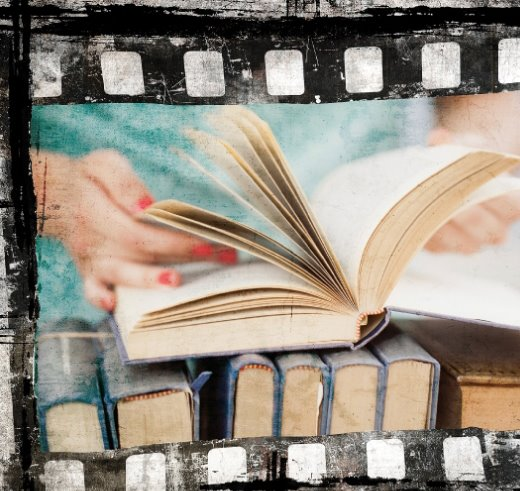
\includegraphics[scale=1.8]{xx.jpg}}} % Image background
\centering
\vspace*{3cm}
\par\normalfont\fontsize{35}{35}\sffamily\selectfont
\textbf{\textcolor{black}{CINELEE}}\\
{\LARGE }\par % Book title
\vspace*{1cm}
{\Huge \fcolorbox{black}{white}{ANGIE TATIANA MOLANO GUZMÁN} }\par
\vspace*{14cm}
{\huge \fcolorbox{black}{white}{\textbf{\textsc{Editorial Maguen David}}} }
% Author name
\endgroup

%----------------------------------------------------------------------------------------
%	COPYRIGHT PAGE
%----------------------------------------------------------------------------------------
\afterpage{\null\newpage}
\newpage
~\vfill
\thispagestyle{empty}


\afterpage{\null\newpage}
\onecolumn
\newpage
\thispagestyle{empty}
\begin{center}
\vspace*{5cm}
\Huge{\textbf{CINELLE\\}}
\vspace*{3cm}
\huge{\textbf{Angie Tatiana Molano Guzmán\\}}
\vspace*{7cm}
\huge{\textsc{Editorial Maguen David}}
\end{center}

\newpage
\thispagestyle{empty}
~\vfill
%\noindent Copyright \copyright\ 2014 Andrea Hidalgo\\ % Copyright notice
%\small
\noindent \textsc{CINELEE}\\\\
\noindent \textsc{Estudiante Universidad Pedagógica Nacional:}  \textit{Angie Tatiana Molano Guzmán}\\
\noindent \textsc{Asesoría pedagógica y editorial:} Docente Universidad Pedagógica Nacional \textit{Leonardo Cano}\\ % License information
\noindent \textsc{Asesoría gráfica:} \textit{Daniel Siervo}\\ % License information
\noindent Publicado en Noviembre de 2017 \\\\ % Printing/edition date 

\noindent \textsc{\textbf{Editorial Maguen David}}\\\\
\noindent \textbf{\small{Todo el material que aparece en la Unidad Didáctica Cinlee está protegido por las Leyes de Propiedad Intelectual vigentes.}}\\\\
\noindent\small{ \textbf{Copyright \copyright\ 2017 Unidad Didáctica Cinelee. Todos los derechos reservados. No se copiará, fotocopiará, reproducirá, traducirá o reducirá con cualquier tipo de medio electrónico o formato legible por máquina, ninguno de los materiales disponibles en la Unidad Didáctica Cinlee, en su totalidad o en parte, sin el consentimiento previo por escrito de la autora Angie Tatiana Molano G.. Toda reproducción, en la forma que se produjese, y sin el permiso de la autora Angie Tatiana Molano G. queda prohibida. Queda asimismo prohibida su distribución con fines comerciales.}}
\large
%----------------------------------------------------------------------------------------
%	TABLE OF CONTENTS
%----------------------------------------------------------------------------------------
\chapterimage{pano-5.jpg} % heading image

\pagestyle{empty} % No headers

\renewcommand\contentsname{Tabla de Contenido}
\renewcommand{\bibname}{Bibliographie}
\tableofcontents% Print the table of contents itself

%\cleardoublepage % Forces the first chapter to start on an odd page so it's on the right

\pagestyle{fancy} % Print headers again

%----------------------------------------------------------------------------------------
%	CHAPTER 1
%----------------------------------------------------------------------------------------
\twocolumn
\chapterimage{pano-5.jpg} % Chapter heading image

\chapter{Poema I}

\section{En el fondo de un poema}\index{poema}

\vspace{2em}

% caja de "En esta lección" 
\begin{theorem}
--
\sffamily
\begin{itemize}
\item Identificarás figuras retóricas dentro de un texto.
\item Comprenderás a fondo un poema. 
\item Analizarás una película.
\item Conectarás un poema con una película.
\item Realizarás un guión literario.
\item Utilizarás adecuadamente los conectores lógicos.
\item Realizarás y expondrás un texto argumentativo. 
\end{itemize}
\end{theorem}

% caja de "sabias que"
\begin{definition}
Las figuras retóricas, también llamadas figuras literarias, representan una manera diferente de utilizar el lenguaje. La finalidad de estas figuras es crear un estilo comunicativo más original, más literario. Las Figuras Retóricas ayudan a captar la atención, sorprenden por su originalidad y poseen un gran poder sugerente y persuasivo permitiendo una comunicación más eficaz. En español existen más de cien figuras retóricas y muchas de ellas son variantes de una misma idea. Las más conocidas son: metáfora, sinonimia, hipérbole, paradoja e ironía. 
\end{definition}

  \vspace{1em}
\subsection*{Instrucción}
El siguiente poema tiene como título “Lista negra” y se encuentran en el libro País Secreto (1988) del autor Juan Manuel Roca. Realiza una primera lectura de este para después realizar una taller relacionado con este. \\

% poema
\textit{\textbf{Lista negra}}

\vspace{0.5em}
\textit{Hago la lista negra de mis dudas en medio de un país diezmado y no sé si las cartas que no llegan son violadas como el sueño o las mujeres...\\
(Al amanecer arrecia la lluvia y acaso la tormenta acalle disparos lejanos...)\\
No sé, exactamente, si algún hombre en mi país es buscado en la ciudad con la oculta lámpara de algún ladrón de sueños...\\
(Alguien al borde de un abismo acaso inicie el retrato hablado de un ángel...)\\
Y cuando llega la noche o entro al sueño como a un tren que me saca de un país oscuro, pienso si algún oculto guardián decidiera aplicarme la ley de fuga de los sueños…\\
\begin{flushright}
Juan Manuel Roca
\end{flushright}
}
\vspace{2em}

\begin{exercise}
-
\begin{itemize}
\item[\textbf{A.}] Del poema:
\item[1.] Escribe las palabras desconocidas y luego busca  su significado en el diccionario. \\
\rule[-0.2mm]{64mm}{0.1mm}
\rule[-0.2mm]{64mm}{0.1mm}
\rule[-0.2mm]{64mm}{0.1mm}
\rule[-0.2mm]{64mm}{0.1mm}
\rule[-0.2mm]{64mm}{0.1mm}
\rule[-0.2mm]{64mm}{0.1mm} \\
\item[\textbf{B.}] Lee de nuevo el poema teniendo en cuenta las palabras que previamente has consultado.\\
\item[\textbf{C.}] De manera general, ¿Qué has entendido del poema hasta el momento? \\
\rule[-0.2mm]{64mm}{0.1mm}
\rule[-0.2mm]{64mm}{0.1mm}
\rule[-0.2mm]{64mm}{0.1mm}
\rule[-0.2mm]{64mm}{0.1mm} \\
\item[\textbf{D.}] Teniendo en cuenta el poema y tus conocimientos, responde:
\item[1.] ¿Por qué el autor del texto describe la lista como negra y no de otro color?\\
\rule[-0.2mm]{64mm}{0.1mm}
\rule[-0.2mm]{64mm}{0.1mm}
\rule[-0.2mm]{64mm}{0.1mm}
\rule[-0.2mm]{64mm}{0.1mm}
\rule[-0.2mm]{64mm}{0.1mm} \\
\item[2.] ¿A qué hace referencia violar una carta?\\
\rule[-0.2mm]{64mm}{0.1mm}
\rule[-0.2mm]{64mm}{0.1mm}
\rule[-0.2mm]{64mm}{0.1mm}
\rule[-0.2mm]{64mm}{0.1mm}
\rule[-0.2mm]{64mm}{0.1mm} \\
\item[3.] ¿Qué imagen te trae la frase “oculta lámpara”? \\
\rule[-0.2mm]{64mm}{0.1mm}
\rule[-0.2mm]{64mm}{0.1mm}
\rule[-0.2mm]{64mm}{0.1mm}
\rule[-0.2mm]{64mm}{0.1mm}
\rule[-0.2mm]{64mm}{0.1mm} \\
\item[4.] ¿En qué situación alguien podría encontrarse “al borde de un abismo”?  \\
\rule[-0.2mm]{64mm}{0.1mm}
\rule[-0.2mm]{64mm}{0.1mm}
\rule[-0.2mm]{64mm}{0.1mm}
\rule[-0.2mm]{64mm}{0.1mm}
\rule[-0.2mm]{64mm}{0.1mm} \\
\item[5.] Si se tiene la idea de un guardián como aquella persona que cuida y protege a un individuo o a un colectivo, ¿Por qué en el texto se habla de un “oculto guardián”?  \\
\rule[-0.2mm]{64mm}{0.1mm}
\rule[-0.2mm]{64mm}{0.1mm}
\rule[-0.2mm]{64mm}{0.1mm}
\rule[-0.2mm]{64mm}{0.1mm}
\rule[-0.2mm]{64mm}{0.1mm} \\
\item[6.] ¿A qué se refiere “la ley de fuga de los sueños”?  \\
\rule[-0.2mm]{64mm}{0.1mm}
\rule[-0.2mm]{64mm}{0.1mm}
\rule[-0.2mm]{64mm}{0.1mm}
\rule[-0.2mm]{64mm}{0.1mm}
\rule[-0.2mm]{64mm}{0.1mm} \\
\item[\textbf{F.}] Describe en un párrafo sobre qué se trata el poema y qué fue lo que más te llamó la atención de este. \\
\rule[-0.2mm]{64mm}{0.1mm}
\rule[-0.2mm]{64mm}{0.1mm}
\rule[-0.2mm]{64mm}{0.1mm}
\rule[-0.2mm]{64mm}{0.1mm}
\rule[-0.2mm]{64mm}{0.1mm}
\rule[-0.2mm]{64mm}{0.1mm}
\rule[-0.2mm]{64mm}{0.1mm}
\rule[-0.2mm]{64mm}{0.1mm}
\rule[-0.2mm]{64mm}{0.1mm}
\rule[-0.2mm]{64mm}{0.1mm}
\rule[-0.2mm]{64mm}{0.1mm}
\rule[-0.2mm]{64mm}{0.1mm}
\rule[-0.2mm]{64mm}{0.1mm}
\rule[-0.2mm]{64mm}{0.1mm}
\rule[-0.2mm]{64mm}{0.1mm} \\
\end{itemize}
\end{exercise}
  \vspace{2em}
  
% -----------------------------------------------------------
%   SECCION #2
% ============================================================

%\chapterimage{pano-5.jpg} % Chapter heading image
%\chapter*{Sección \# 2: En el fondo de una película}
\section{En el fondo de una película}
% caja de "sabias que"
\begin{definition}
Silencio en el paraíso (2011) muestra, a través de una historia de amor juvenil, el caso de los falsos positivos, como se conoce en Colombia el asesinato por miembros del ejército de civiles inocentes para hacerlos pasar como guerrilleros muertos en combate. Además de ser dirigida por Colbert García, ha sido la ganadora de la Biznaga de Plata al mejor largometraje en la sección Territorio Latinoamericano del decimoquinto Festival de Cine Español de Málaga, en el sur de España. 
\end{definition}

\vspace{1em}
\subsection*{Instrucción}
A continuación vas a ver la película “El silencio en el paraíso” de Colbert García, que se encuentra en el CD de la unidad didáctica bajo el título de la película. Observa cuidadosamente cómo se desarrollan los siguientes aspectos en la película:\\
\begin{itemize}
\item Posibilidades de trabajo en la ciudad
\item Sueños (proyectos, ambiciones) en los protagonistas
\item Pobreza
\item Drogas
\item Violencia en el barrio
\end{itemize}

\vspace{2em}

\begin{exercise}
Después de haber visto la película “Silencio en el paraíso” realizaremos la siguiente actividad, ésta con el propósito de generar una crítica con respecto a la película,  y así mismo una relación entre esta y el poema “Lista negra” visto en la sección 1.1. \textit{En el fondo de un poema} \\
\begin{itemize}
\item[\textbf{A.}] Teniendo en cuenta los aspectos que se señalaron antes de ver la película (Posibilidades de trabajo en la ciudad, sueños, pobreza, drogas, violencia en el barrio) describe de una manera muy general qué pasa en la película.
\rule[-0.2mm]{64mm}{0.1mm}
\rule[-0.2mm]{64mm}{0.1mm}
\rule[-0.2mm]{64mm}{0.1mm}
\rule[-0.2mm]{64mm}{0.1mm}
\rule[-0.2mm]{64mm}{0.1mm}
\rule[-0.2mm]{64mm}{0.1mm}
\rule[-0.2mm]{64mm}{0.1mm}
\rule[-0.2mm]{64mm}{0.1mm} \\
\item[\textbf{B.}] Teniendo en cuenta el tercer verso del poema “Lista negra” de Juan M. Roca:\\\\
\textit{“No sé, exactamente, si algún hombre en mi país es buscado en la ciudad con la oculta lámpara de algún ladrón de sueños…”}
\\\\
En la película ¿Quiénes o qué cosas son los ladrones de sueños y cuáles son sus ocultas lámparas? \\
\rule[-0.2mm]{64mm}{0.1mm}
\rule[-0.2mm]{64mm}{0.1mm}
\rule[-0.2mm]{64mm}{0.1mm}
\rule[-0.2mm]{64mm}{0.1mm}
\rule[-0.2mm]{64mm}{0.1mm}
\rule[-0.2mm]{64mm}{0.1mm} \\
\item[\textbf{C.}] A través de un guión literario recrea UNA de las siguientes situaciones, usa los personajes que requieras e incluso ve más allá de lo que simplemente muestra la película. Puedes también utilizar fragmentos del poema antes visto. \\\\
\begin{itemize}
\item[$\bullet$] Extorsión por parte del grupo de la torre (negro, carlos) hacía los comerciantes del barrio El Paraíso.
\item[$\bullet$] Robo de la bicicleta de Ronald.
\item[$\bullet$] Trabajo de doña Susana.
\item[$\bullet$] Trabajo de los militares.
\item[$\bullet$] Situación de Leidy en su casa.
\item[$\bullet$] Lectura de la carta que le da Ronald a Leidy.
\item[$\bullet$] Coqueteo entre doña Susana y Ronald.
\item[$\bullet$] Propuesta de Yeison (el gordo) a Ronald de robar.
\item[$\bullet$] Muerte de los jóvenes que iban a trabajar fuera de la ciudad.

\end{itemize}

\end{itemize}
\end{exercise}


% caja "Para tener en cuenta"
\begin{corollary}
En el guión literario se incluye la división por escenas, las acciones de los personajes o hechos del relato, el diálogo entre personajes, breves descripciones del entorno o escenario en el que van a suceder los hechos. Un guión literario da información suficiente para imaginar la película: expresa cómo se hacen los diálogos, cómo actúan los personajes, en qué escenarios actúan y con qué objetos interactúan, sin especificar todavía los detalles de la producción. 
\end{corollary}


\textbf{Guión literario} \\
\rule[-0.2mm]{76mm}{0.1mm}
\rule[-0.2mm]{76mm}{0.1mm}
\rule[-0.2mm]{76mm}{0.1mm}
\rule[-0.2mm]{76mm}{0.1mm}
\rule[-0.2mm]{76mm}{0.1mm}
\rule[-0.2mm]{76mm}{0.1mm}
\rule[-0.2mm]{76mm}{0.1mm}
\rule[-0.2mm]{76mm}{0.1mm}
\rule[-0.2mm]{76mm}{0.1mm}
\rule[-0.2mm]{76mm}{0.1mm}
\rule[-0.2mm]{76mm}{0.1mm}
\rule[-0.2mm]{76mm}{0.1mm}
\rule[-0.2mm]{76mm}{0.1mm}
\rule[-0.2mm]{76mm}{0.1mm}
\rule[-0.2mm]{76mm}{0.1mm}
\rule[-0.2mm]{76mm}{0.1mm}
\rule[-0.2mm]{76mm}{0.1mm}
\rule[-0.2mm]{76mm}{0.1mm}
\rule[-0.2mm]{76mm}{0.1mm}
\rule[-0.2mm]{76mm}{0.1mm}
\rule[-0.2mm]{76mm}{0.1mm}
\rule[-0.2mm]{76mm}{0.1mm}
\vspace{2em}


% -----------------------------------------------------------
%   SECCION #3
% ============================================================


%\chapterimage{pano-5.jpg} % Chapter heading image
%\chapter{Sección \# 3: Mi texto, mi argumento}
\section{Mi texto, mi argumento}
% caja de "sabias que"
\begin{definition}
Los conectores son palabras o grupos de palabras que sirven para evidenciar la relación entre dos ideas. Estas relaciones pueden darse entre enunciados de una misma oración, entre oraciones o entre párrafos. Expresar adecuadamente la relación entre nuestras ideas le permite al lector encontrarle sentido al texto. Algunos ejemplos son:  
\end{definition}

\vspace{1em}

%--------------------
% tabla
\begin{table}[h]
\small\sffamily
\centering
\begin{tabular}{cl}
\rowcolor[HTML]{E1DBDB} 
\textbf{Tipo} & \multicolumn{1}{c}{\cellcolor[HTML]{E1DBDB}\textbf{Conectores}} \\ \hline
\rowcolor[HTML]{FFFFFF} 
\textbf{\begin{tabular}[c]{@{}c@{}}Relación de \\ adición\end{tabular}} & \begin{tabular}[c]{@{}l@{}}“y”,”además”, “más aún”. \\ “todavía más”, “incluso”, \\ “aparte”, “encima”, “después”, \\ “de igual forma”, “también”, \\ “por otra parte”, \\ “por otro lado”, \\ “así mismo (o asimismo)”, etc.\end{tabular} \\
\rowcolor[HTML]{E1DBDB} 
\textbf{\begin{tabular}[c]{@{}c@{}}Relación \\ temporal\end{tabular}} & \begin{tabular}[c]{@{}l@{}}“primero”, “luego”, \\ “entonces”, “a continuación”, \\ antes”, “pronto”, “antes que”, \\ “después de”, \\ “al mismo tiempo”,\\ ”desde hace...”, \\ “hasta hace...”, etc.\end{tabular} \\
\textbf{\begin{tabular}[c]{@{}c@{}}Relación \\ de causa\end{tabular}} & \begin{tabular}[c]{@{}l@{}}Se usan para introducir, \\ como su nombre lo dice, \\ la causa o motivo de una \\ circunstancia o suceso. \\ Entre ellos encontramos: \\ Porque, pues, ya que, \\ debido a que, dado que.\end{tabular}\\
\rowcolor[HTML]{E1DBDB} 
\textbf{\begin{tabular}[c]{@{}c@{}}Relación de \\ consecuencia\end{tabular}} & \begin{tabular}[c]{@{}l@{}}A diferencia de los anteriores, \\ estos conectores introducen el \\ resultado o consecuencia de un \\ suceso o acción. \\ Entre ellos están: Por eso, \\ por lo tanto, en consecuencia, \\ de esta manera, \\ por consiguiente, así pues, \\ de modo que, de manera que, \\ entonces.\end{tabular} \\
\textbf{\begin{tabular}[c]{@{}c@{}}Relación \\ adversativa\end{tabular}} & \begin{tabular}[c]{@{}l@{}}“pero”, “aunque” “a pesar de que”,\\ ”sin embargo”, “no obstante”, \\ “por otra parte” “aun así”, etc.\end{tabular} 
\end{tabular}
\end{table}

\begin{table}[h]
\small\sffamily
\centering
\begin{tabular}{cl}
\rowcolor[HTML]{E1DBDB} 
\textbf{\begin{tabular}[c]{@{}c@{}}Relación \\ de explicación\end{tabular}} & \begin{tabular}[c]{@{}l@{}}“es decir”, o sea”, “esto es”, \\ “a saber”, “o lo que es lo mismo”, \\ “en otras palabras”, \\ “mejor dicho”, etc.\end{tabular} \\
\textbf{\begin{tabular}[c]{@{}c@{}}Construcción \\ de hipótesis\end{tabular}} & “si (entonces)...” \\
\rowcolor[HTML]{E1DBDB} 
\textbf{\begin{tabular}[c]{@{}c@{}}Relación \\ de cierre \\ o conclusión\end{tabular}} & \begin{tabular}[c]{@{}l@{}}Finalmente, en conclusión, \\ en síntesis, por último, \\ en resumen, etc.\end{tabular}
\end{tabular}
\end{table}

\newpage
\subsection*{Instrucción}
Teniendo en cuenta los talleres de las sesiones anteriores y la relación entre la película y el poema, realiza un texto argumentativo o un cuento donde se evidencia tu postura y opinión sobre: pobreza, drogas, violencia, posibilidades de trabajo y sueños en los habitantes de la ciudad de Bogotá. Ten en cuenta las siguientes indicaciones:

\begin{itemize}
\item Extensión: 3 - 4 párrafos
\item Escrito a mano o digital
\end{itemize}
% ----------------------------------------------------------------------------------------
% 	BIBLIOGRAPHY
% ----------------------------------------------------------------------------------------
\begin{comment}
\begin{thebibliography}{9}

  \bibitem{1}
           Alain F.Zuur, Elena N.Ieno, Neil J.Walker, Anatoly A.Saveliev, Graham M.Smith,
          \emph{Mixed Effects and Extensions in Ecology with R}.
          Springer,
          129-142,
          2009.            
          
       \bibitem{3}
           Laurent DAVEZIES,
          \emph{Modèles à effets fixes, à effets aléatoires, modèles mixtes ou multi-niveaux :
propriétés et mises en oeuvre des modélisations
de l’hétérogénéité dans le cas de données groupées}.
          60-70,
          G 2011 / 03.
 \url{http://www.crest.fr/ckfinder/userfiles/files/Pageperso/ldavezies/WorkingPaperINSEE/G2011-03.pdf}
 
\end{thebibliography}
\end{comment}


\end{document}